\documentclass[pdf]{ifacconf}


\usepackage{amsmath}
\usepackage{natbib}            % you should have natbib.sty
\usepackage{graphicx}          % Include this line if your 
                               % document contains figures,
%\usepackage[dvips]{epsfig}    % or this line, depending on which
                               % you prefer.
                               
\usepackage{units}
%\usepackage{babelbib}
%\bibliographystyle{babunsrt}

% for German
\usepackage{ngerman}           % neue Deutsche Rechtschreibung, Silbentrennung
\usepackage[UTF8]{inputenc}  % Eingabe von Umlaute im Editor
%\usepackage[T1]{fontenc}       % Trennung mit Umlauten

\usepackage{tikz,pgfplots}
\pgfplotsset{compat=newest} 
\usetikzlibrary{shapes,arrows,positioning,arrows.meta}


\begin{document}

\begin{frontmatter}

\title{``Projektwettbewerb Einführung in die Regelungstechnik'' - Stabilisierung eines
Segways auf einer
Wippe}

%\thanks[footnoteinfo]{Institute for Systems Theory and Automatic Control, University of Stuttgart, Germany. \textit{http://www.ist.uni-stuttgart.de}}

% include all authors, underline corresponding author
%\author{\underline{},} 
\author{Alessio Gaggiano, Shadi Rafe, Truc-Quynh Doan} 
% \author{}

\begin{abstract}\\                          % Abstract of not more than 250 words.
Die folgende Dokumentation beinhaltet die ausführliche Beschreibung unseres Lösungsansatzes der regelungstechnischen Aufgabe ``Stabilisierung eines Segways auf einer Wippe''. 
%This is a template for the laboratory course ``Projektwettbewerb Einführung in die Regelungstechnik'' at the Institute for Systems Theory and Automatic Control, University of Stuttgart. Use this document to write your report with \LaTeX\ (cf. \cite{Knuth2005}).
\end{abstract}

\end{frontmatter}

\section{Motivation}
%We have designed a state feedback for the single-track model based on inverse kinematics, loop-shaping, feedback linearization, and robot navigation functions.

Die uns gestellte Regelungsaufgabe verlangte eine Stabilisierung eines Segways auf einer Wippe, die durch ein Feder-Dämpfer-System gelagert wird und mit einem Helligkeitsverlauf versehen ist. Dabei soll das Segway eine Sollposition halten. 


\section{Lösungsansatz}
%Our design procedure was based on the idea that accelerating a vehicle results in shorter lap times than braking a vehicle. For presentational conciseness, we have listed some important parameters in Table 1.

%Modellierung => Linearisierung
%sechs Zustände
%Stabilität => Zustandsrückführung
%LQR-Regler
%Regler mit nichtlinearen System zusammengeschaltet
%Pole vorgebbar => Beobachter, da nicht alle Zustände messbar
%Lueberger Beobachter 
%Zustandsrückführung mit Beobachter verbinden 
%Regelaweichung => Vorfilter

Die uns vorliegende Modellierung des Regelsystems ist nichtlinear, daher erlaubte dies uns keine einfache Implementierung einer Regelung nach den uns bekannten Methoden der Vorlesung ``Einführung in die Regelungstechnik''. Eine Linearisierung des Systems ist nötig.





\begin{table}[h]
\caption{Important Parameters.}
\label{table:working plan}
\centering
\begin{tabular}{|c|c|}
\hline
\bfseries Parameter & \bfseries Value \\ \hline \hline
lap time $t_{\text{f}}$ & $\infty$ \\ \hline
control gain $k$ & $0$ \\ \hline
steering angle $\delta$ & $-\left( e^{i \pi}+1\right)$ \\ \hline
 \end{tabular}
\end{table}

\section{Fazit}
We have achieved a lap time of $t_{\text{f}}=\infty$. We have depicted a plot of vehicle velocity $v$ versus an independent curve parameter $\gamma$, with which we have parameterized the racetrack, in Fig. 1. 

\begin{figure}[h] % use \begin{figure*} for two-column figure
\begin{center}
% This file was created by matlab2tikz.
%
%The latest updates can be retrieved from
%  http://www.mathworks.com/matlabcentral/fileexchange/22022-matlab2tikz-matlab2tikz
%where you can also make suggestions and rate matlab2tikz.
%
\definecolor{mycolor1}{rgb}{0.00000,0.44700,0.74100}%
\definecolor{mycolor2}{rgb}{0.85000,0.32500,0.09800}%
%
\begin{tikzpicture}
\pgfplotsset{scale only axis,
xmin=0,
xmax=400,}

\begin{axis}[%
width=.35\textwidth,
height=3.5cm,
xlabel={time in min},
ylabel={\textcolor{mycolor1}{signal strength}},
ymin=-0.006,
ymax=0.006,
axis y line*=left,
every y tick/.style={mycolor1},
yticklabel style = {mycolor1}
]
\addplot [color=mycolor1,solid,thick]
  table[row sep=crcr]{%
0	0.0001\\
1.00250626566416	0.0001\\
2.00501253132832	0.0001\\
3.00751879699248	0.0001\\
4.01002506265664	0.0001\\
5.0125313283208	0.0001\\
6.01503759398496	0.0001\\
7.01754385964912	0.0001\\
8.02005012531328	0.0001\\
9.02255639097744	0.0001\\
10.0250626566416	0.0001\\
11.0275689223058	0.0001\\
12.0300751879699	0.0001\\
13.0325814536341	0.0001\\
14.0350877192982	0.0001\\
15.0375939849624	0.0001\\
16.0401002506266	0.0001\\
17.0426065162907	0.0001\\
18.0451127819549	0.0001\\
19.047619047619	0.0001\\
20.0501253132832	0.0001\\
21.0526315789474	0.0001\\
22.0551378446115	0.0001\\
23.0576441102757	0.0001\\
24.0601503759398	0.0001\\
25.062656641604	0.000103132832080201\\
26.0651629072682	0.000153258145363409\\
27.0676691729323	0.000203383458646617\\
28.0701754385965	0.000253508771929824\\
29.0726817042607	0.000303634085213033\\
30.0751879699248	0.000353759398496241\\
31.077694235589	0.000403884711779449\\
32.0802005012531	0.000454010025062657\\
33.0827067669173	0.000504135338345865\\
34.0852130325815	0.000554260651629073\\
35.0877192982456	0.000604385964912281\\
36.0902255639098	0.000654511278195489\\
37.0927318295739	0.000704636591478697\\
38.0952380952381	0.000754761904761905\\
39.0977443609023	0.000804887218045113\\
40.1002506265664	0.000855012531328321\\
41.1027568922306	0.000905137844611529\\
42.1052631578947	0.000955263157894737\\
43.1077694235589	0.00100538847117795\\
44.1102756892231	0.00105551378446115\\
45.1127819548872	0.00110563909774436\\
46.1152882205514	0.00115576441102757\\
47.1177944862155	0.00120588972431078\\
48.1203007518797	0.00125601503759398\\
49.1228070175439	0.00130614035087719\\
50.125313283208	0.0013562656641604\\
51.1278195488722	0.00140639097744361\\
52.1303258145363	0.00145651629072682\\
53.1328320802005	0.00150664160401003\\
54.1353383458647	0.00155676691729323\\
55.1378446115288	0.00160689223057644\\
56.140350877193	0.00165701754385965\\
57.1428571428571	0.00170714285714286\\
58.1453634085213	0.00175726817042607\\
59.1478696741855	0.00180739348370927\\
60.1503759398496	0.00185751879699248\\
61.1528822055138	0.00190764411027569\\
62.1553884711779	0.0019577694235589\\
63.1578947368421	0.00200789473684211\\
64.1604010025063	0.00205802005012531\\
65.1629072681704	0.00210814536340852\\
66.1654135338346	0.00215827067669173\\
67.1679197994987	0.00220839598997494\\
68.1704260651629	0.00225852130325815\\
69.1729323308271	0.00230864661654135\\
70.1754385964912	0.00235877192982456\\
71.1779448621554	0.00240889724310777\\
72.1804511278196	0.00245902255639098\\
73.1829573934837	0.00250914786967419\\
74.1854636591479	0.00255927318295739\\
75.187969924812	0.0026\\
76.1904761904762	0.0026\\
77.1929824561404	0.0026\\
78.1954887218045	0.0026\\
79.1979949874687	0.0026\\
80.2005012531328	0.0026\\
81.203007518797	0.0026\\
82.2055137844611	0.0026\\
83.2080200501253	0.0026\\
84.2105263157895	0.0026\\
85.2130325814536	0.0026\\
86.2155388471178	0.0026\\
87.218045112782	0.0026\\
88.2205513784461	0.0026\\
89.2230576441103	0.0026\\
90.2255639097744	0.0026\\
91.2280701754386	0.0026\\
92.2305764411028	0.0026\\
93.2330827067669	0.0026\\
94.2355889724311	0.0026\\
95.2380952380952	0.0026\\
96.2406015037594	0.0026\\
97.2431077694236	0.0026\\
98.2456140350877	0.0026\\
99.2481203007519	0.0026\\
100.250626566416	0.0026\\
101.25313283208	0.0026\\
102.255639097744	0.0026\\
103.258145363409	0.0026\\
104.260651629073	0.0026\\
105.263157894737	0.0026\\
106.265664160401	0.0026\\
107.268170426065	0.0026\\
108.270676691729	0.0026\\
109.273182957393	0.0026\\
110.275689223058	0.0026\\
111.278195488722	0.0026\\
112.280701754386	0.0026\\
113.28320802005	0.0026\\
114.285714285714	0.0026\\
115.288220551378	0.0026\\
116.290726817043	0.0026\\
117.293233082707	0.0026\\
118.295739348371	0.0026\\
119.298245614035	0.0026\\
120.300751879699	0.0026\\
121.303258145363	0.0026\\
122.305764411028	0.0026\\
123.308270676692	0.0026\\
124.310776942356	0.0026\\
125.31328320802	0.002584335839599\\
126.315789473684	0.00253421052631579\\
127.318295739348	0.00248408521303258\\
128.320802005013	0.00243395989974937\\
129.323308270677	0.00238383458646616\\
130.325814536341	0.00233370927318296\\
131.328320802005	0.00228358395989975\\
132.330827067669	0.00223345864661654\\
133.333333333333	0.00218333333333333\\
134.335839598998	0.00213320802005013\\
135.338345864662	0.00208308270676692\\
136.340852130326	0.00203295739348371\\
137.34335839599	0.0019828320802005\\
138.345864661654	0.00193270676691729\\
139.348370927318	0.00188258145363409\\
140.350877192982	0.00183245614035088\\
141.353383458647	0.00178233082706767\\
142.355889724311	0.00173220551378446\\
143.358395989975	0.00168208020050125\\
144.360902255639	0.00163195488721804\\
145.363408521303	0.00158182957393484\\
146.365914786967	0.00153170426065163\\
147.368421052632	0.00148157894736842\\
148.370927318296	0.00143145363408521\\
149.37343358396	0.00138132832080201\\
150.375939849624	0.0013312030075188\\
151.378446115288	0.00128107769423559\\
152.380952380952	0.00123095238095238\\
153.383458646617	0.00118082706766917\\
154.385964912281	0.00113070175438596\\
155.388471177945	0.00108057644110276\\
156.390977443609	0.00103045112781955\\
157.393483709273	0.000980325814536342\\
158.395989974937	0.000930200501253132\\
159.398496240602	0.000880075187969925\\
160.401002506266	0.000829949874686717\\
161.40350877193	0.000779824561403508\\
162.406015037594	0.000729699248120301\\
163.408521303258	0.000679573934837093\\
164.411027568922	0.000629448621553885\\
165.413533834586	0.000579323308270676\\
166.416040100251	0.000529197994987469\\
167.418546365915	0.000479072681704261\\
168.421052631579	0.000428947368421052\\
169.423558897243	0.000378822055137844\\
170.426065162907	0.000328696741854637\\
171.428571428571	0.000278571428571429\\
172.431077694236	0.00022844611528822\\
173.4335839599	0.000178320802005013\\
174.436090225564	0.000128195488721805\\
175.438596491228	0.0001\\
176.441102756892	0.0001\\
177.443609022556	0.0001\\
178.446115288221	0.0001\\
179.448621553885	0.0001\\
180.451127819549	0.0001\\
181.453634085213	0.0001\\
182.456140350877	0.0001\\
183.458646616541	0.0001\\
184.461152882206	0.0001\\
185.46365914787	0.0001\\
186.466165413534	0.0001\\
187.468671679198	0.0001\\
188.471177944862	0.0001\\
189.473684210526	0.0001\\
190.47619047619	0.0001\\
191.478696741855	0.0001\\
192.481203007519	0.0001\\
193.483709273183	0.0001\\
194.486215538847	0.0001\\
195.488721804511	0.0001\\
196.491228070175	0.0001\\
197.49373433584	0.0001\\
198.496240601504	0.0001\\
199.498746867168	0.0001\\
200.501253132832	0.0001\\
201.503759398496	0.0001\\
202.50626566416	0.0001\\
203.508771929825	0.0001\\
204.511278195489	0.0001\\
205.513784461153	0.0001\\
206.516290726817	0.0001\\
207.518796992481	0.0001\\
208.521303258145	0.0001\\
209.52380952381	0.0001\\
210.526315789474	0.0001\\
211.528822055138	0.0001\\
212.531328320802	0.0001\\
213.533834586466	0.0001\\
214.53634085213	0.0001\\
215.538847117794	0.0001\\
216.541353383459	0.0001\\
217.543859649123	0.0001\\
218.546365914787	0.0001\\
219.548872180451	0.0001\\
220.551378446115	0.0001\\
221.553884711779	0.0001\\
222.556390977444	0.0001\\
223.558897243108	0.0001\\
224.561403508772	0.0001\\
225.563909774436	0.00015639097744361\\
226.5664160401	0.000256641604010025\\
227.568922305764	0.00035689223057644\\
228.571428571429	0.000457142857142858\\
229.573934837093	0.000557393483709274\\
230.576441102757	0.000657644110275689\\
231.578947368421	0.000757894736842104\\
232.581453634085	0.000858145363408522\\
233.583959899749	0.000958395989974937\\
234.586466165414	0.00105864661654135\\
235.588972431078	0.00115889724310777\\
236.591478696742	0.00125914786967419\\
237.593984962406	0.0013593984962406\\
238.59649122807	0.00145964912280702\\
239.598997493734	0.00155989974937343\\
240.601503759399	0.00166015037593985\\
241.604010025063	0.00176040100250626\\
242.606516290727	0.00186065162907268\\
243.609022556391	0.0019609022556391\\
244.611528822055	0.00206115288220551\\
245.614035087719	0.00216140350877193\\
246.616541353383	0.00226165413533835\\
247.619047619048	0.00236190476190476\\
248.621553884712	0.00246215538847118\\
249.624060150376	0.0025624060150376\\
250.62656641604	0.00266265664160401\\
251.629072681704	0.00276290726817043\\
252.631578947368	0.00286315789473684\\
253.634085213033	0.00296340852130326\\
254.636591478697	0.00306365914786967\\
255.639097744361	0.00316390977443609\\
256.641604010025	0.00326416040100251\\
257.644110275689	0.00336441102756892\\
258.646616541353	0.00346466165413534\\
259.649122807018	0.00356491228070175\\
260.651629072682	0.00366516290726817\\
261.654135338346	0.00376541353383458\\
262.65664160401	0.003865664160401\\
263.659147869674	0.00396591478696742\\
264.661654135338	0.00406616541353383\\
265.664160401003	0.00416641604010025\\
266.666666666667	0.00426666666666667\\
267.669172932331	0.00436691729323308\\
268.671679197995	0.0044671679197995\\
269.674185463659	0.00456741854636592\\
270.676691729323	0.00466766917293233\\
271.679197994987	0.00476791979949875\\
272.681704260652	0.00486817042606517\\
273.684210526316	0.00496842105263158\\
274.68671679198	0.005068671679198\\
275.689223057644	0.0051\\
276.691729323308	0.0051\\
277.694235588972	0.0051\\
278.696741854637	0.0051\\
279.699248120301	0.0051\\
280.701754385965	0.0051\\
281.704260651629	0.0051\\
282.706766917293	0.0051\\
283.709273182957	0.0051\\
284.711779448622	0.0051\\
285.714285714286	0.0051\\
286.71679197995	0.0051\\
287.719298245614	0.0051\\
288.721804511278	0.0051\\
289.724310776942	0.0051\\
290.726817042607	0.0051\\
291.729323308271	0.0051\\
292.731829573935	0.0051\\
293.734335839599	0.0051\\
294.736842105263	0.0051\\
295.739348370927	0.0051\\
296.741854636591	0.0051\\
297.744360902256	0.0051\\
298.74686716792	0.0051\\
299.749373433584	0.0051\\
300.751879699248	0.0051\\
301.754385964912	0.0051\\
302.756892230576	0.0051\\
303.759398496241	0.0051\\
304.761904761905	0.0051\\
305.764411027569	0.0051\\
306.766917293233	0.0051\\
307.769423558897	0.0051\\
308.771929824561	0.0051\\
309.774436090226	0.0051\\
310.77694235589	0.0051\\
311.779448621554	0.0051\\
312.781954887218	0.0051\\
313.784461152882	0.0051\\
314.786967418546	0.0051\\
315.789473684211	0.0051\\
316.791979949875	0.0051\\
317.794486215539	0.0051\\
318.796992481203	0.0051\\
319.799498746867	0.0051\\
320.802005012531	0.0051\\
321.804511278195	0.0051\\
322.80701754386	0.0051\\
323.809523809524	0.0051\\
324.812030075188	0.0051\\
325.814536340852	0.00501854636591478\\
326.817042606516	0.00491829573934837\\
327.81954887218	0.00481804511278195\\
328.822055137845	0.00471779448621554\\
329.824561403509	0.00461754385964912\\
330.827067669173	0.00451729323308271\\
331.829573934837	0.00441704260651629\\
332.832080200501	0.00431679197994988\\
333.834586466165	0.00421654135338346\\
334.83709273183	0.00411629072681704\\
335.839598997494	0.00401604010025063\\
336.842105263158	0.00391578947368421\\
337.844611528822	0.0038155388471178\\
338.847117794486	0.00371528822055138\\
339.84962406015	0.00361503759398496\\
340.852130325815	0.00351478696741855\\
341.854636591479	0.00341453634085213\\
342.857142857143	0.00331428571428572\\
343.859649122807	0.0032140350877193\\
344.862155388471	0.00311378446115288\\
345.864661654135	0.00301353383458647\\
346.8671679198	0.00291328320802005\\
347.869674185464	0.00281303258145363\\
348.872180451128	0.00271278195488722\\
349.874686716792	0.0026125313283208\\
350.877192982456	0.00251228070175438\\
351.87969924812	0.00241203007518797\\
352.882205513784	0.00231177944862155\\
353.884711779449	0.00221152882205514\\
354.887218045113	0.00211127819548872\\
355.889724310777	0.0020110275689223\\
356.892230576441	0.00191077694235589\\
357.894736842105	0.00181052631578947\\
358.897243107769	0.00171027568922306\\
359.899749373434	0.00161002506265664\\
360.902255639098	0.00150977443609023\\
361.904761904762	0.00140952380952381\\
362.907268170426	0.0013092731829574\\
363.90977443609	0.00120902255639098\\
364.912280701754	0.00110877192982456\\
365.914786967419	0.00100852130325815\\
366.917293233083	0.000908270676691728\\
367.919799498747	0.000808020050125316\\
368.922305764411	0.000707769423558898\\
369.924812030075	0.00060751879699248\\
370.927318295739	0.000507268170426067\\
371.929824561404	0.000407017543859649\\
372.932330827068	0.000306766917293231\\
373.934837092732	0.000206516290726819\\
374.937343358396	0.000106265664160401\\
375.93984962406	0.0001\\
376.942355889724	0.0001\\
377.944862155388	0.0001\\
378.947368421053	0.0001\\
379.949874686717	0.0001\\
380.952380952381	0.0001\\
381.954887218045	0.0001\\
382.957393483709	0.0001\\
383.959899749373	0.0001\\
384.962406015038	0.0001\\
385.964912280702	0.0001\\
386.967418546366	0.0001\\
387.96992481203	0.0001\\
388.972431077694	0.0001\\
389.974937343358	0.0001\\
390.977443609023	0.0001\\
391.979949874687	0.0001\\
392.982456140351	0.0001\\
393.984962406015	0.0001\\
394.987468671679	0.0001\\
395.989974937343	0.0001\\
396.992481203008	0.0001\\
397.994987468672	0.0001\\
398.997493734336	0.0001\\
400	0.0001\\
};\label{plot_one}
\end{axis}

\begin{axis}[%
width=.35\textwidth,
height=3.5cm,
%at={(0.758in,0.481in)},
%scale only axis,
%xmin=0,
%xmax=400,
ymin=-1.5,
ymax=1.5,
ylabel={\textcolor{mycolor2}{normalized amount}},
axis y line*=right,
yticklabel pos=right,
ytick={-1,0,1},
yticklabels={-20,0,20},
legend style={at={(axis cs:20,-1.47)},anchor=south west,legend cell align=left,align=left,fill=none,draw=none},
every y tick/.style={mycolor2},
yticklabel style = {mycolor2}
]
\addlegendimage{/pgfplots/refstyle=plot_one}\addlegendentry{$u(t)$}
\addplot [color=mycolor2,solid,dashed,thick]
  table[row sep=crcr]{%
0	0\\
1.00250626566416	0\\
2.00501253132832	0\\
3.00751879699248	0\\
4.01002506265664	0\\
5.0125313283208	0\\
6.01503759398496	0\\
7.01754385964912	0\\
8.02005012531328	0\\
9.02255639097744	0\\
10.0250626566416	0\\
11.0275689223058	0\\
12.0300751879699	0\\
13.0325814536341	0\\
14.0350877192982	0\\
15.0375939849624	0\\
16.0401002506266	0\\
17.0426065162907	0\\
18.0451127819549	0\\
19.047619047619	0\\
20.0501253132832	0\\
21.0526315789474	0\\
22.0551378446115	0\\
23.0576441102757	0\\
24.0601503759398	0\\
25.062656641604	0.0312500000000004\\
26.0651629072682	0.499999999999997\\
27.0676691729323	0.499999999999997\\
28.0701754385965	0.499999999999997\\
29.0726817042607	0.499999999999997\\
30.0751879699248	0.499999999999997\\
31.077694235589	0.499999999999997\\
32.0802005012531	0.499999999999997\\
33.0827067669173	0.499999999999997\\
34.0852130325815	0.499999999999997\\
35.0877192982456	0.499999999999997\\
36.0902255639098	0.499999999999997\\
37.0927318295739	0.499999999999996\\
38.0952380952381	0.499999999999997\\
39.0977443609023	0.499999999999997\\
40.1002506265664	0.499999999999996\\
41.1027568922306	0.499999999999997\\
42.1052631578947	0.499999999999997\\
43.1077694235589	0.499999999999997\\
44.1102756892231	0.499999999999997\\
45.1127819548872	0.499999999999997\\
46.1152882205514	0.499999999999995\\
47.1177944862155	0.499999999999997\\
48.1203007518797	0.499999999999997\\
49.1228070175439	0.499999999999998\\
50.125313283208	0.499999999999995\\
51.1278195488722	0.499999999999997\\
52.1303258145363	0.499999999999997\\
53.1328320802005	0.499999999999997\\
54.1353383458647	0.499999999999997\\
55.1378446115288	0.499999999999997\\
56.140350877193	0.499999999999997\\
57.1428571428571	0.499999999999996\\
58.1453634085213	0.499999999999997\\
59.1478696741855	0.499999999999997\\
60.1503759398496	0.499999999999997\\
61.1528822055138	0.499999999999995\\
62.1553884711779	0.5\\
63.1578947368421	0.499999999999995\\
64.1604010025063	0.499999999999995\\
65.1629072681704	0.5\\
66.1654135338346	0.499999999999994\\
67.1679197994987	0.5\\
68.1704260651629	0.499999999999996\\
69.1729323308271	0.499999999999994\\
70.1754385964912	0.5\\
71.1779448621554	0.499999999999994\\
72.1804511278196	0.499999999999996\\
73.1829573934837	0.499999999999999\\
74.1854636591479	0.499999999999996\\
75.187969924812	0.406250000000004\\
76.1904761904762	0\\
77.1929824561404	0\\
78.1954887218045	0\\
79.1979949874687	0\\
80.2005012531328	0\\
81.203007518797	0\\
82.2055137844611	0\\
83.2080200501253	0\\
84.2105263157895	0\\
85.2130325814536	0\\
86.2155388471178	0\\
87.218045112782	0\\
88.2205513784461	0\\
89.2230576441103	0\\
90.2255639097744	0\\
91.2280701754386	0\\
92.2305764411028	0\\
93.2330827067669	0\\
94.2355889724311	0\\
95.2380952380952	0\\
96.2406015037594	0\\
97.2431077694236	0\\
98.2456140350877	0\\
99.2481203007519	0\\
100.250626566416	0\\
101.25313283208	0\\
102.255639097744	0\\
103.258145363409	0\\
104.260651629073	0\\
105.263157894737	0\\
106.265664160401	0\\
107.268170426065	0\\
108.270676691729	0\\
109.273182957393	0\\
110.275689223058	0\\
111.278195488722	0\\
112.280701754386	0\\
113.28320802005	0\\
114.285714285714	0\\
115.288220551378	0\\
116.290726817043	0\\
117.293233082707	0\\
118.295739348371	0\\
119.298245614035	0\\
120.300751879699	0\\
121.303258145363	0\\
122.305764411028	0\\
123.308270676692	0\\
124.310776942356	0\\
125.31328320802	-0.15625\\
126.315789473684	-0.499999999999999\\
127.318295739348	-0.499999999999996\\
128.320802005013	-0.499999999999999\\
129.323308270677	-0.499999999999998\\
130.325814536341	-0.499999999999994\\
131.328320802005	-0.499999999999999\\
132.330827067669	-0.499999999999999\\
133.333333333333	-0.499999999999993\\
134.335839598998	-0.499999999999999\\
135.338345864662	-0.499999999999999\\
136.340852130326	-0.499999999999993\\
137.34335839599	-0.499999999999999\\
138.345864661654	-0.499999999999997\\
139.348370927318	-0.499999999999999\\
140.350877192982	-0.499999999999995\\
141.353383458647	-0.499999999999999\\
142.355889724311	-0.499999999999997\\
143.358395989975	-0.499999999999997\\
144.360902255639	-0.499999999999998\\
145.363408521303	-0.499999999999997\\
146.365914786967	-0.499999999999997\\
147.368421052632	-0.499999999999998\\
148.370927318296	-0.499999999999997\\
149.37343358396	-0.499999999999997\\
150.375939849624	-0.499999999999999\\
151.378446115288	-0.499999999999995\\
152.380952380952	-0.499999999999997\\
153.383458646617	-0.499999999999999\\
154.385964912281	-0.499999999999995\\
155.388471177945	-0.499999999999999\\
156.390977443609	-0.499999999999997\\
157.393483709273	-0.499999999999997\\
158.395989974937	-0.499999999999998\\
159.398496240602	-0.499999999999997\\
160.401002506266	-0.499999999999998\\
161.40350877193	-0.499999999999997\\
162.406015037594	-0.499999999999997\\
163.408521303258	-0.499999999999998\\
164.411027568922	-0.499999999999997\\
165.413533834586	-0.499999999999998\\
166.416040100251	-0.499999999999997\\
167.418546365915	-0.499999999999997\\
168.421052631579	-0.499999999999997\\
169.423558897243	-0.499999999999997\\
170.426065162907	-0.499999999999997\\
171.428571428571	-0.499999999999997\\
172.431077694236	-0.499999999999997\\
173.4335839599	-0.499999999999997\\
174.436090225564	-0.499999999999997\\
175.438596491228	-0.281249999999997\\
176.441102756892	0\\
177.443609022556	0\\
178.446115288221	0\\
179.448621553885	0\\
180.451127819549	0\\
181.453634085213	0\\
182.456140350877	0\\
183.458646616541	0\\
184.461152882206	0\\
185.46365914787	0\\
186.466165413534	0\\
187.468671679198	0\\
188.471177944862	0\\
189.473684210526	0\\
190.47619047619	0\\
191.478696741855	0\\
192.481203007519	0\\
193.483709273183	0\\
194.486215538847	0\\
195.488721804511	0\\
196.491228070175	0\\
197.49373433584	0\\
198.496240601504	0\\
199.498746867168	0\\
200.501253132832	0\\
201.503759398496	0\\
202.50626566416	0\\
203.508771929825	0\\
204.511278195489	0\\
205.513784461153	0\\
206.516290726817	0\\
207.518796992481	0\\
208.521303258145	0\\
209.52380952381	0\\
210.526315789474	0\\
211.528822055138	0\\
212.531328320802	0\\
213.533834586466	0\\
214.53634085213	0\\
215.538847117794	0\\
216.541353383459	0\\
217.543859649123	0\\
218.546365914787	0\\
219.548872180451	0\\
220.551378446115	0\\
221.553884711779	0\\
222.556390977444	0\\
223.558897243108	0\\
224.561403508772	0\\
225.563909774436	0.562499999999993\\
226.5664160401	0.999999999999994\\
227.568922305764	0.999999999999994\\
228.571428571429	0.999999999999994\\
229.573934837093	0.999999999999994\\
230.576441102757	0.999999999999994\\
231.578947368421	0.999999999999994\\
232.581453634085	0.999999999999994\\
233.583959899749	0.999999999999994\\
234.586466165414	0.999999999999993\\
235.588972431078	0.999999999999995\\
236.591478696742	0.999999999999993\\
237.593984962406	0.999999999999995\\
238.59649122807	0.999999999999993\\
239.598997493734	0.999999999999995\\
240.601503759399	0.999999999999993\\
241.604010025063	0.999999999999993\\
242.606516290727	0.999999999999995\\
243.609022556391	0.999999999999995\\
244.611528822055	0.999999999999993\\
245.614035087719	0.999999999999993\\
246.616541353383	0.999999999999995\\
247.619047619048	0.999999999999993\\
248.621553884712	0.999999999999993\\
249.624060150376	0.999999999999995\\
250.62656641604	0.999999999999993\\
251.629072681704	0.999999999999993\\
252.631578947368	0.999999999999998\\
253.634085213033	0.999999999999991\\
254.636591478697	0.999999999999998\\
255.639097744361	0.999999999999993\\
256.641604010025	0.999999999999993\\
257.644110275689	0.999999999999995\\
258.646616541353	0.999999999999995\\
259.649122807018	0.999999999999991\\
260.651629072682	0.999999999999995\\
261.654135338346	0.999999999999996\\
262.65664160401	0.999999999999991\\
263.659147869674	0.999999999999995\\
264.661654135338	0.999999999999991\\
265.664160401003	0.999999999999995\\
266.666666666667	0.999999999999995\\
267.669172932331	1\\
268.671679197995	0.999999999999987\\
269.674185463659	0.999999999999995\\
270.676691729323	1\\
271.679197994987	0.999999999999987\\
272.681704260652	0.999999999999995\\
273.684210526316	1\\
274.68671679198	0.999999999999995\\
275.689223057644	0.312499999999996\\
276.691729323308	0\\
277.694235588972	0\\
278.696741854637	0\\
279.699248120301	0\\
280.701754385965	0\\
281.704260651629	0\\
282.706766917293	0\\
283.709273182957	0\\
284.711779448622	0\\
285.714285714286	0\\
286.71679197995	0\\
287.719298245614	0\\
288.721804511278	0\\
289.724310776942	0\\
290.726817042607	0\\
291.729323308271	0\\
292.731829573935	0\\
293.734335839599	0\\
294.736842105263	0\\
295.739348370927	0\\
296.741854636591	0\\
297.744360902256	0\\
298.74686716792	0\\
299.749373433584	0\\
300.751879699248	0\\
301.754385964912	0\\
302.756892230576	0\\
303.759398496241	0\\
304.761904761905	0\\
305.764411027569	0\\
306.766917293233	0\\
307.769423558897	0\\
308.771929824561	0\\
309.774436090226	0\\
310.77694235589	0\\
311.779448621554	0\\
312.781954887218	0\\
313.784461152882	0\\
314.786967418546	0\\
315.789473684211	0\\
316.791979949875	0\\
317.794486215539	0\\
318.796992481203	0\\
319.799498746867	0\\
320.802005012531	0\\
321.804511278195	0\\
322.80701754386	0\\
323.809523809524	0\\
324.812030075188	0\\
325.814536340852	-0.81250000000001\\
326.817042606516	-0.999999999999991\\
327.81954887218	-0.999999999999995\\
328.822055137845	-0.999999999999991\\
329.824561403509	-0.999999999999995\\
330.827067669173	-0.999999999999995\\
331.829573934837	-0.999999999999991\\
332.832080200501	-0.999999999999995\\
333.834586466165	-0.999999999999995\\
334.83709273183	-0.999999999999991\\
335.839598997494	-0.999999999999995\\
336.842105263158	-0.999999999999995\\
337.844611528822	-0.999999999999996\\
338.847117794486	-0.999999999999995\\
339.84962406015	-0.999999999999991\\
340.852130325815	-0.999999999999996\\
341.854636591479	-0.999999999999995\\
342.857142857143	-0.999999999999991\\
343.859649122807	-0.999999999999995\\
344.862155388471	-0.999999999999995\\
345.864661654135	-0.999999999999996\\
346.8671679198	-0.999999999999991\\
347.869674185464	-0.999999999999995\\
348.872180451128	-0.999999999999996\\
349.874686716792	-0.999999999999995\\
350.877192982456	-0.999999999999991\\
351.87969924812	-0.999999999999996\\
352.882205513784	-0.999999999999995\\
353.884711779449	-0.999999999999991\\
354.887218045113	-0.999999999999995\\
355.889724310777	-0.999999999999995\\
356.892230576441	-0.999999999999993\\
357.894736842105	-0.999999999999995\\
358.897243107769	-0.999999999999993\\
359.899749373434	-0.999999999999996\\
360.902255639098	-0.999999999999993\\
361.904761904762	-0.999999999999995\\
362.907268170426	-0.999999999999993\\
363.90977443609	-0.999999999999993\\
364.912280701754	-0.999999999999995\\
365.914786967419	-0.999999999999993\\
366.917293233083	-0.999999999999995\\
367.919799498747	-0.999999999999993\\
368.922305764411	-0.999999999999994\\
369.924812030075	-0.999999999999994\\
370.927318295739	-0.999999999999995\\
371.929824561404	-0.999999999999994\\
372.932330827068	-0.999999999999994\\
373.934837092732	-0.999999999999994\\
374.937343358396	-0.999999999999994\\
375.93984962406	-0.0624999999999961\\
376.942355889724	0\\
377.944862155388	0\\
378.947368421053	0\\
379.949874686717	0\\
380.952380952381	0\\
381.954887218045	0\\
382.957393483709	0\\
383.959899749373	0\\
384.962406015038	0\\
385.964912280702	0\\
386.967418546366	0\\
387.96992481203	0\\
388.972431077694	0\\
389.974937343358	0\\
390.977443609023	0\\
391.979949874687	0\\
392.982456140351	0\\
393.984962406015	0\\
394.987468671679	0\\
395.989974937343	0\\
396.992481203008	0\\
397.994987468672	0\\
398.997493734336	0\\
400	0\\
};
\addlegendentry{$\dot{u}_{\text{norm}}(t)$};

\addplot [color=mycolor2,thick]
  table[row sep=crcr]{%
0	-0.00636588364106934\\
1.00250626566416	-0.00636588363688404\\
2.00501253132832	-0.00636588363451691\\
3.00751879699248	-0.00636588363333856\\
4.01002506265664	-0.00636588363312632\\
5.0125313283208	-0.00636588363300764\\
6.01503759398496	-0.00636588363353805\\
7.01754385964912	-0.00636588363471717\\
8.02005012531328	-0.00636588363505389\\
9.02255639097744	-0.00636588363522477\\
10.0250626566416	-0.00636588363557077\\
11.0275689223058	-0.00636588363609268\\
12.0300751879699	-0.00636588363679049\\
13.0325814536341	-0.00636588363766381\\
14.0350877192982	-0.00636588363871265\\
15.0375939849624	-0.00636588363954731\\
16.0401002506266	-0.00636588364006883\\
17.0426065162907	-0.00636588364044885\\
18.0451127819549	-0.00636588364069666\\
19.047619047619	-0.0063658836408312\\
20.0501253132832	-0.00636588364083931\\
21.0526315789474	-0.00636588364072218\\
22.0551378446115	-0.00636588364054937\\
23.0576441102757	-0.00636588364038313\\
24.0601503759398	-0.00636588364022617\\
25.062656641604	-0.00636588364005762\\
26.0651629072682	-0.00618445709412547\\
27.0676691729323	0.00348808129421098\\
28.0701754385965	0.0363025757871417\\
29.0726817042607	0.0886242585138117\\
30.0751879699248	0.148051351136587\\
31.077694235589	0.206907966072253\\
32.0802005012531	0.263254845322584\\
33.0827067669173	0.316742535779687\\
34.0852130325815	0.363555178837958\\
35.0877192982456	0.400259798485863\\
36.0902255639098	0.426772090207529\\
37.0927318295739	0.44455919129173\\
38.0952380952381	0.455583761192601\\
39.0977443609023	0.461734846945584\\
40.1002506265664	0.464594425821516\\
41.1027568922306	0.465393291401035\\
42.1052631578947	0.465026011013084\\
43.1077694235589	0.464095198223395\\
44.1102756892231	0.462976557916776\\
45.1127819548872	0.461890223377085\\
46.1152882205514	0.460955943368565\\
47.1177944862155	0.460225479297758\\
48.1203007518797	0.459703029490724\\
49.1228070175439	0.459364512447151\\
50.125313283208	0.459175739221298\\
51.1278195488722	0.459104180119856\\
52.1303258145363	0.459122456359267\\
53.1328320802005	0.459204239233681\\
54.1353383458647	0.459329640759907\\
55.1378446115288	0.459483888325746\\
56.140350877193	0.459656489948973\\
57.1428571428571	0.45984043576963\\
58.1453634085213	0.460031477439891\\
59.1478696741855	0.46022721157928\\
60.1503759398496	0.460426571178644\\
61.1528822055138	0.460629575636956\\
62.1553884711779	0.460836868694713\\
63.1578947368421	0.461049258342043\\
64.1604010025063	0.461268298073307\\
65.1629072681704	0.461495385592135\\
66.1654135338346	0.461732291601299\\
67.1679197994987	0.461981063976831\\
68.1704260651629	0.462243914696503\\
69.1729323308271	0.462523385767151\\
70.1754385964912	0.462822376966719\\
71.1779448621554	0.46314419268064\\
72.1804511278196	0.463492612572291\\
73.1829573934837	0.463871853739652\\
74.1854636591479	0.46428657204828\\
75.187969924812	0.464741823980795\\
76.1904761904762	0.464938538725563\\
77.1929824561404	0.455425726373276\\
78.1954887218045	0.425115115524885\\
79.1979949874687	0.37722504593297\\
80.2005012531328	0.319944410683753\\
81.203007518797	0.260936444563986\\
82.2055137844611	0.205608693111183\\
83.2080200501253	0.157065838768606\\
84.2105263157895	0.11658273584713\\
85.2130325814536	0.0841969368154859\\
86.2155388471178	0.0592155373380268\\
87.218045112782	0.0405799563181548\\
88.2205513784461	0.0271136722639005\\
89.2230576441103	0.0177023569614258\\
90.2255639097744	0.0113706373951291\\
91.2280701754386	0.00729361163148866\\
92.2305764411028	0.00480827215919559\\
93.2330827067669	0.00340882736432331\\
94.2355889724311	0.0027233308394641\\
95.2380952380952	0.00248676625715336\\
96.2406015037594	0.00251803420886689\\
97.2431077694236	0.00268660683164934\\
98.2456140350877	0.00290844889090301\\
99.2481203007519	0.00313437292940968\\
100.250626566416	0.00333927532304384\\
101.25313283208	0.00351401045316773\\
102.255639097744	0.00365665617237762\\
103.258145363409	0.00376810943042441\\
104.260651629073	0.0038514405698332\\
105.263157894737	0.00391097909562262\\
106.265664160401	0.00395173979480785\\
107.268170426065	0.00397908177647619\\
108.270676691729	0.00399703582652384\\
109.273182957393	0.00400900663932723\\
110.275689223058	0.00401605290981708\\
111.278195488722	0.00402105075041305\\
112.280701754386	0.00402251964676104\\
113.28320802005	0.00402302452746864\\
114.285714285714	0.00402138957659446\\
115.288220551378	0.00401905803630295\\
116.290726817043	0.00401657086656898\\
117.293233082707	0.00401406582697503\\
118.295739348371	0.00401247156996133\\
119.298245614035	0.00401064106302592\\
120.300751879699	0.00400932753903965\\
121.303258145363	0.00400898730445293\\
122.305764411028	0.00400894125569826\\
123.308270676692	0.00400890243160162\\
124.310776942356	0.0040092694277539\\
125.31328320802	0.00401006634082054\\
126.315789473684	0.00336699229294166\\
127.318295739348	-0.00919651572588334\\
128.320802005013	-0.0430566084361201\\
129.323308270677	-0.0937946215606562\\
130.325814536341	-0.152967564830019\\
131.328320802005	-0.213047289876659\\
132.330827067669	-0.268849768177623\\
133.333333333333	-0.31748799202831\\
134.335839598998	-0.357888466802174\\
135.338345864662	-0.390157130408343\\
136.340852130326	-0.415072921822991\\
137.34335839599	-0.433753525346257\\
138.345864661654	-0.44739594998896\\
139.348370927318	-0.45711588188194\\
140.350877192982	-0.46388413588478\\
141.353383458647	-0.468500032701935\\
142.355889724311	-0.471590691415146\\
143.358395989975	-0.473630663762118\\
144.360902255639	-0.474967289445048\\
145.363408521303	-0.475848965320988\\
146.365914786967	-0.476448753302804\\
147.368421052632	-0.476882288708269\\
148.370927318296	-0.477223244114127\\
149.37343358396	-0.477516116398913\\
150.375939849624	-0.477787099447263\\
151.378446115288	-0.47805038757822\\
152.380952380952	-0.47831231144553\\
153.383458646617	-0.478574854844438\\
154.385964912281	-0.478837815114297\\
155.388471177945	-0.479099818179086\\
156.390977443609	-0.479359376162907\\
157.393483709273	-0.479615056218843\\
158.395989974937	-0.479865778752911\\
159.398496240602	-0.480110852494685\\
160.401002506266	-0.480349940747527\\
161.40350877193	-0.480582958393482\\
162.406015037594	-0.480810092907075\\
163.408521303258	-0.481031639354135\\
164.411027568922	-0.481248016013192\\
165.413533834586	-0.48145969356985\\
166.416040100251	-0.481667117417815\\
167.418546365915	-0.481870779420153\\
168.421052631579	-0.482071067024849\\
169.423558897243	-0.482268224420485\\
170.426065162907	-0.482462880670978\\
171.428571428571	-0.482655306047184\\
172.431077694236	-0.482845665555577\\
173.4335839599	-0.483034200448403\\
174.436090225564	-0.483221189836379\\
175.438596491228	-0.483406794710097\\
176.441102756892	-0.482043886205149\\
177.443609022556	-0.464471693028379\\
178.446115288221	-0.42326396387683\\
179.448621553885	-0.365036799655494\\
180.451127819549	-0.299604195294792\\
181.453634085213	-0.235180306246125\\
182.456140350877	-0.177157591009115\\
183.458646616541	-0.128273393215538\\
184.461152882206	-0.089288494225277\\
185.46365914787	-0.0596684093420011\\
186.466165413534	-0.0381800121271256\\
187.468671679198	-0.0233301173290723\\
188.471177944862	-0.0136131697285193\\
189.473684210526	-0.0076699251118358\\
190.47619047619	-0.00437370067905226\\
191.478696741855	-0.00284766079618571\\
192.481203007519	-0.00243320189297956\\
193.483709273183	-0.00265214344440226\\
194.486215538847	-0.00317829313164509\\
195.488721804511	-0.00380775128140194\\
196.491228070175	-0.0044239156247426\\
197.49373433584	-0.00496600446572628\\
198.496240601504	-0.00540830220599001\\
199.498746867168	-0.00574797154822392\\
200.501253132832	-0.0059957902479627\\
201.503759398496	-0.00616808455992477\\
202.50626566416	-0.00628147573494487\\
203.508771929825	-0.00635088981643726\\
204.511278195489	-0.00638916866566193\\
205.513784461153	-0.00640680378270405\\
206.516290726817	-0.00641168321705456\\
207.518796992481	-0.00640926909817947\\
208.521303258145	-0.00640318583334912\\
209.52380952381	-0.00639580011669631\\
210.526315789474	-0.00638857571624535\\
211.528822055138	-0.00638226359179379\\
212.531328320802	-0.0063771316181775\\
213.533834586466	-0.0063731503704784\\
214.53634085213	-0.00637020354140574\\
215.538847117794	-0.0063680827584306\\
216.541353383459	-0.00636668386692104\\
217.543859649123	-0.00636582097815383\\
218.546365914787	-0.00636526994351091\\
219.548872180451	-0.00636490732359518\\
220.551378446115	-0.00636477704874761\\
221.553884711779	-0.00636476852132688\\
222.556390977444	-0.00636462926456292\\
223.558897243108	-0.00636459499428726\\
224.561403508772	-0.00636480912898825\\
225.563909774436	-0.00636507749600102\\
226.5664160401	-0.00130448702523762\\
227.568922305764	0.0386837120315605\\
228.571428571429	0.111211658243799\\
229.573934837093	0.198927317899813\\
230.576441102757	0.293058008021375\\
231.578947368421	0.389592097051874\\
232.581453634085	0.486678064077109\\
233.583959899749	0.583486652888786\\
234.586466165414	0.679646046260068\\
235.588972431078	0.774980915320599\\
236.591478696742	0.866029040235239\\
237.593984962406	0.936331921282366\\
238.59649122807	0.979032981756825\\
239.598997493734	0.997932552077836\\
240.601503759399	1\\
241.604010025063	0.991908552237377\\
242.606516290727	0.978854020251164\\
243.609022556391	0.96440203619625\\
244.611528822055	0.950715068353665\\
245.614035087719	0.93891222186368\\
246.616541353383	0.929418444119042\\
247.619047619048	0.922226878082106\\
248.621553884712	0.917103789075972\\
249.624060150376	0.913726753616122\\
250.62656641604	0.911767662430113\\
251.629072681704	0.910941615544344\\
252.631578947368	0.911030197057689\\
253.634085213033	0.911888543727399\\
254.636591478697	0.913438830069671\\
255.639097744361	0.91565466031811\\
256.641604010025	0.918530814928059\\
257.644110275689	0.922045045363772\\
258.646616541353	0.926124752177001\\
259.649122807018	0.930632946375667\\
260.651629072682	0.935383491649402\\
261.654135338346	0.940174013040583\\
262.65664160401	0.944820762909043\\
263.659147869674	0.949178865583215\\
264.661654135338	0.953152885456053\\
265.664160401003	0.956691741620186\\
266.666666666667	0.959784189692872\\
267.669172932331	0.962446376211649\\
268.671679197995	0.964713272583808\\
269.674185463659	0.966631303715713\\
270.676691729323	0.968249270727443\\
271.679197994987	0.969618108915175\\
272.681704260652	0.970782455382804\\
273.684210526316	0.971784396111233\\
274.68671679198	0.972653617091462\\
275.689223057644	0.969194262318967\\
276.691729323308	0.942346277703371\\
277.694235588972	0.874317489547944\\
278.696741854637	0.769584755196289\\
279.699248120301	0.644949502367745\\
280.701754385965	0.517094230903704\\
281.704260651629	0.398191214300524\\
282.706766917293	0.295336313764564\\
283.709273182957	0.211398073565865\\
284.711779448622	0.146277671696482\\
285.714285714286	0.0980910744421413\\
286.71679197995	0.064096049845176\\
287.719298245614	0.0413658504178958\\
288.721804511278	0.0270862753655987\\
289.724310776942	0.0187730654091549\\
290.726817042607	0.014556278969166\\
291.729323308271	0.0129872697912293\\
292.731829573935	0.0130009658099975\\
293.734335839599	0.0138543134813029\\
294.736842105263	0.0150510995864512\\
295.739348370927	0.0162867457302841\\
296.741854636591	0.0174248969073047\\
297.744360902256	0.0183869125712799\\
298.74686716792	0.0191453863035306\\
299.749373433584	0.0197107810750297\\
300.751879699248	0.0201119441101529\\
301.754385964912	0.0203821333527197\\
302.756892230576	0.020552094350064\\
303.759398496241	0.0206504658657904\\
304.761904761905	0.0207000553493507\\
305.764411027569	0.020719562118253\\
306.766917293233	0.0207216107827064\\
307.769423558897	0.0207141859923035\\
308.771929824561	0.0207021415875452\\
309.774436090226	0.0206880979026046\\
310.77694235589	0.0206746264481633\\
311.779448621554	0.0206619618312799\\
312.781954887218	0.0206513821804635\\
313.784461152882	0.0206430468089429\\
314.786967418546	0.0206369722170944\\
315.789473684211	0.020633036653719\\
316.791979949875	0.0206305148802119\\
317.794486215539	0.0206293785243875\\
318.796992481203	0.0206289395260188\\
319.799498746867	0.0206285757282862\\
320.802005012531	0.0206286247477596\\
321.804511278195	0.0206284077259751\\
322.80701754386	0.0206281621182585\\
323.809523809524	0.0206278753115527\\
324.812030075188	0.0206276367777995\\
325.814536340852	0.0206194205497724\\
326.817042606516	0.0188730635664032\\
327.81954887218	0.00992443133583895\\
328.822055137845	-0.0204542558083501\\
329.824561403509	-0.074048592213117\\
330.827067669173	-0.145311829906339\\
331.829573934837	-0.228270116004887\\
332.832080200501	-0.318413048730298\\
333.834586466165	-0.412674816912789\\
334.83709273183	-0.50912980089993\\
335.839598997494	-0.606607023166432\\
336.842105263158	-0.704417649323727\\
337.844611528822	-0.802147722726726\\
338.847117794486	-0.899530098622005\\
339.84962406015	-0.996387825737708\\
340.852130325815	-1.08838591140838\\
341.854636591479	-1.15124495695721\\
342.857142857143	-1.174984499898\\
343.859649122807	-1.16700205437046\\
344.862155388471	-1.13911997893235\\
345.864661654135	-1.10189047896592\\
346.8671679198	-1.06294082706625\\
347.869674185464	-1.02695778357097\\
348.872180451128	-0.99632305092297\\
349.874686716792	-0.971822916460135\\
350.877192982456	-0.953261976640126\\
351.87969924812	-0.939937439662945\\
352.882205513784	-0.930951368572268\\
353.884711779449	-0.925409765054204\\
354.887218045113	-0.922527369005122\\
355.889724310777	-0.921675931042218\\
356.892230576441	-0.922387451275335\\
357.894736842105	-0.924333454969435\\
358.897243107769	-0.927280057726639\\
359.899749373434	-0.931035867886436\\
360.902255639098	-0.935406990415643\\
361.904761904762	-0.940175791181411\\
362.907268170426	-0.945109061440161\\
363.90977443609	-0.949990318421898\\
364.912280701754	-0.954627051883261\\
365.914786967419	-0.958895310824267\\
366.917293233083	-0.962702169450646\\
367.919799498747	-0.966023464281568\\
368.922305764411	-0.968854315667573\\
369.924812030075	-0.971222260786315\\
370.927318295739	-0.973187826649981\\
371.929824561404	-0.974776541053868\\
372.932330827068	-0.976067180852719\\
373.934837092732	-0.97709733591486\\
374.937343358396	-0.977927504976271\\
375.93984962406	-0.978491685775248\\
376.942355889724	-0.964327652526008\\
377.944862155388	-0.905102222891981\\
378.947368421053	-0.803007430855355\\
379.949874686717	-0.67613598207367\\
380.952380952381	-0.543096233703334\\
381.954887218045	-0.417728232062084\\
382.957393483709	-0.308231826359396\\
383.959899749373	-0.218152266333653\\
384.962406015038	-0.147687013230534\\
385.964912280702	-0.0950773710403458\\
386.967418546366	-0.0575834815806191\\
387.96992481203	-0.0321478470851668\\
388.972431077694	-0.0158650690246594\\
389.974937343358	-0.00620924498646249\\
390.977443609023	-0.00111812887351966\\
391.979949874687	0.000997258081323361\\
392.982456140351	0.00130471895359262\\
393.984962406015	0.000621578591564199\\
394.987468671679	-0.000510912655899341\\
395.989974937343	-0.00175646413324816\\
396.992481203008	-0.00292454812276223\\
397.994987468672	-0.00392288550384669\\
398.997493734336	-0.00472184201285931\\
400	-0.00532831519357586\\
};
\addlegendentry{$y_{\text{norm}}(t)$};

\end{axis}
\end{tikzpicture}%
\caption{Some arbitrary plot (using tikz) which doesn't have anything to do with Projektwettbewerb ERT.}
\label{fig1}
\end{center}
\end{figure}

\begin{figure}[h] % use \begin{figure*} for two-column figure
\begin{center}
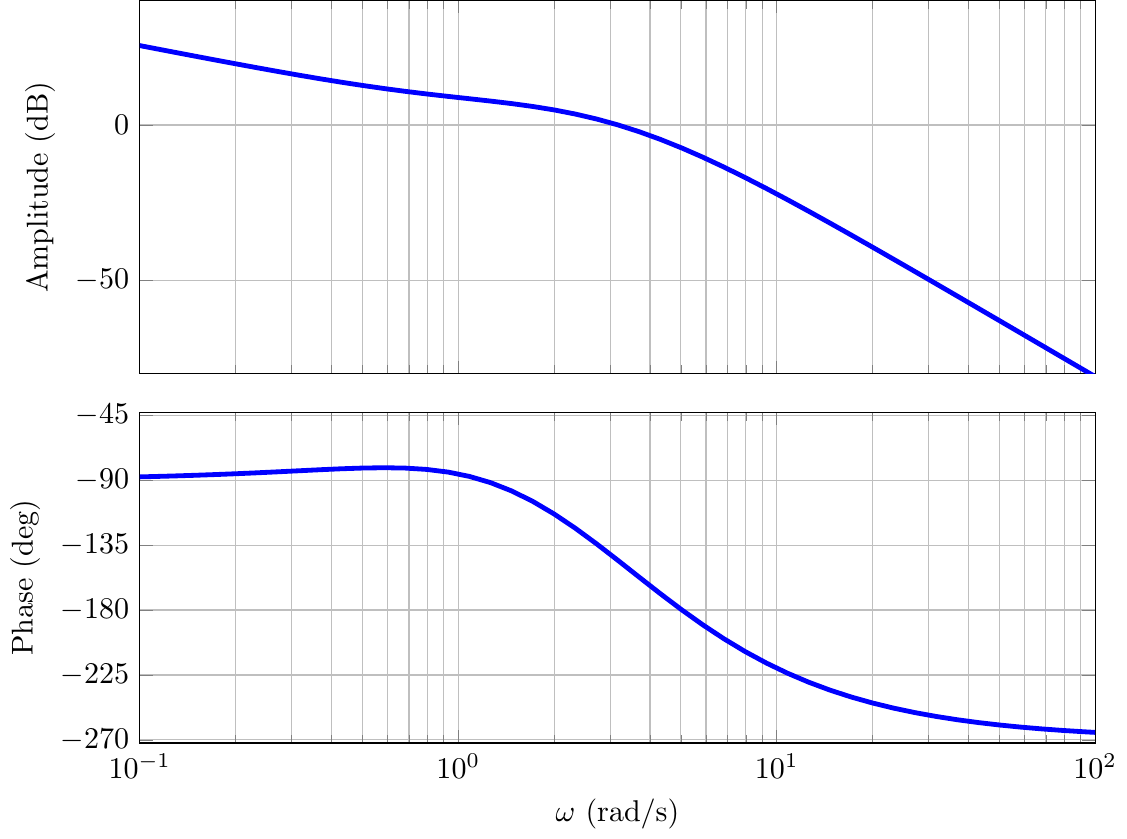
\includegraphics[width=.8\columnwidth]{bode} % inclusion of pdf or png
\caption{Some arbitrary plot (using png) which doesn't have anything to do with Projektwettbewerb ERT.}
\label{fig1}
\end{center}
\end{figure}


\bibliography{Literatur}


%\begin{thebibliography}{3}
%
%\bibitem[(Knuth2005)]{Knuth2005}
%Knuth,~D.~E. (2005).
%\newblock The Art of Computer Programming.
%\newblock Pearson Education.
%
%\end{thebibliography}

%\appendix
\end{document}